\documentclass[11pt, titlepage]{article}

\usepackage[a4paper, margin=1in]{geometry}
\usepackage{graphicx}
\usepackage{tabularx}
\usepackage{float}

\newcolumntype{L}{>{\raggedright\arraybackslash}X}

\author{\textbf{The Terminal}}

\title{\textbf{Coast Capital Contractor Records Database System - Internal Design Doc}}

\begin{document}

\maketitle

\tableofcontents

\clearpage

\section{Introduction}

\subsection{Overview}

The aim of our project is to simplify the system Coast Capital uses for capturing contractor data. Their current system requires tedious manual data entry and complex spreadsheet manipulation, and we want to provide a better method of visualization, management and maintenance. We will be building an online web application designed for ease of use and powerful data analysis. The application aims to make it a straightforward process to add, edit, and visualize contractor data.

\subsection{Goals}

Our application will be easy to learn for new users such that there is not a long ramp-up period for using it in comparison to using excel spreadsheets. Furthermore, since our application is an online web tool, all the contractor data within it will always be the most up to date data available so no two users are viewing different data. The goal will be to implement the following features: a data filtering system, reports visualization, the ability to add or edit contractor data, and an admin panel for admin-specific tasks.

\subsection{Assumptions}

\begin{enumerate}
    \item An admin does not require a filtering method for the various tables that they can access.
    \item The FX table can be updated every 24 hours.
    \item An admin can add as many skills as they want in the skills table.
\end{enumerate}

\section{UI Design}

\subsection{Mock-Up Screens}

The wireframes in this document provides a horizontal wireframe with some vertical functionalities to show the system flow from the eyes of the user. 

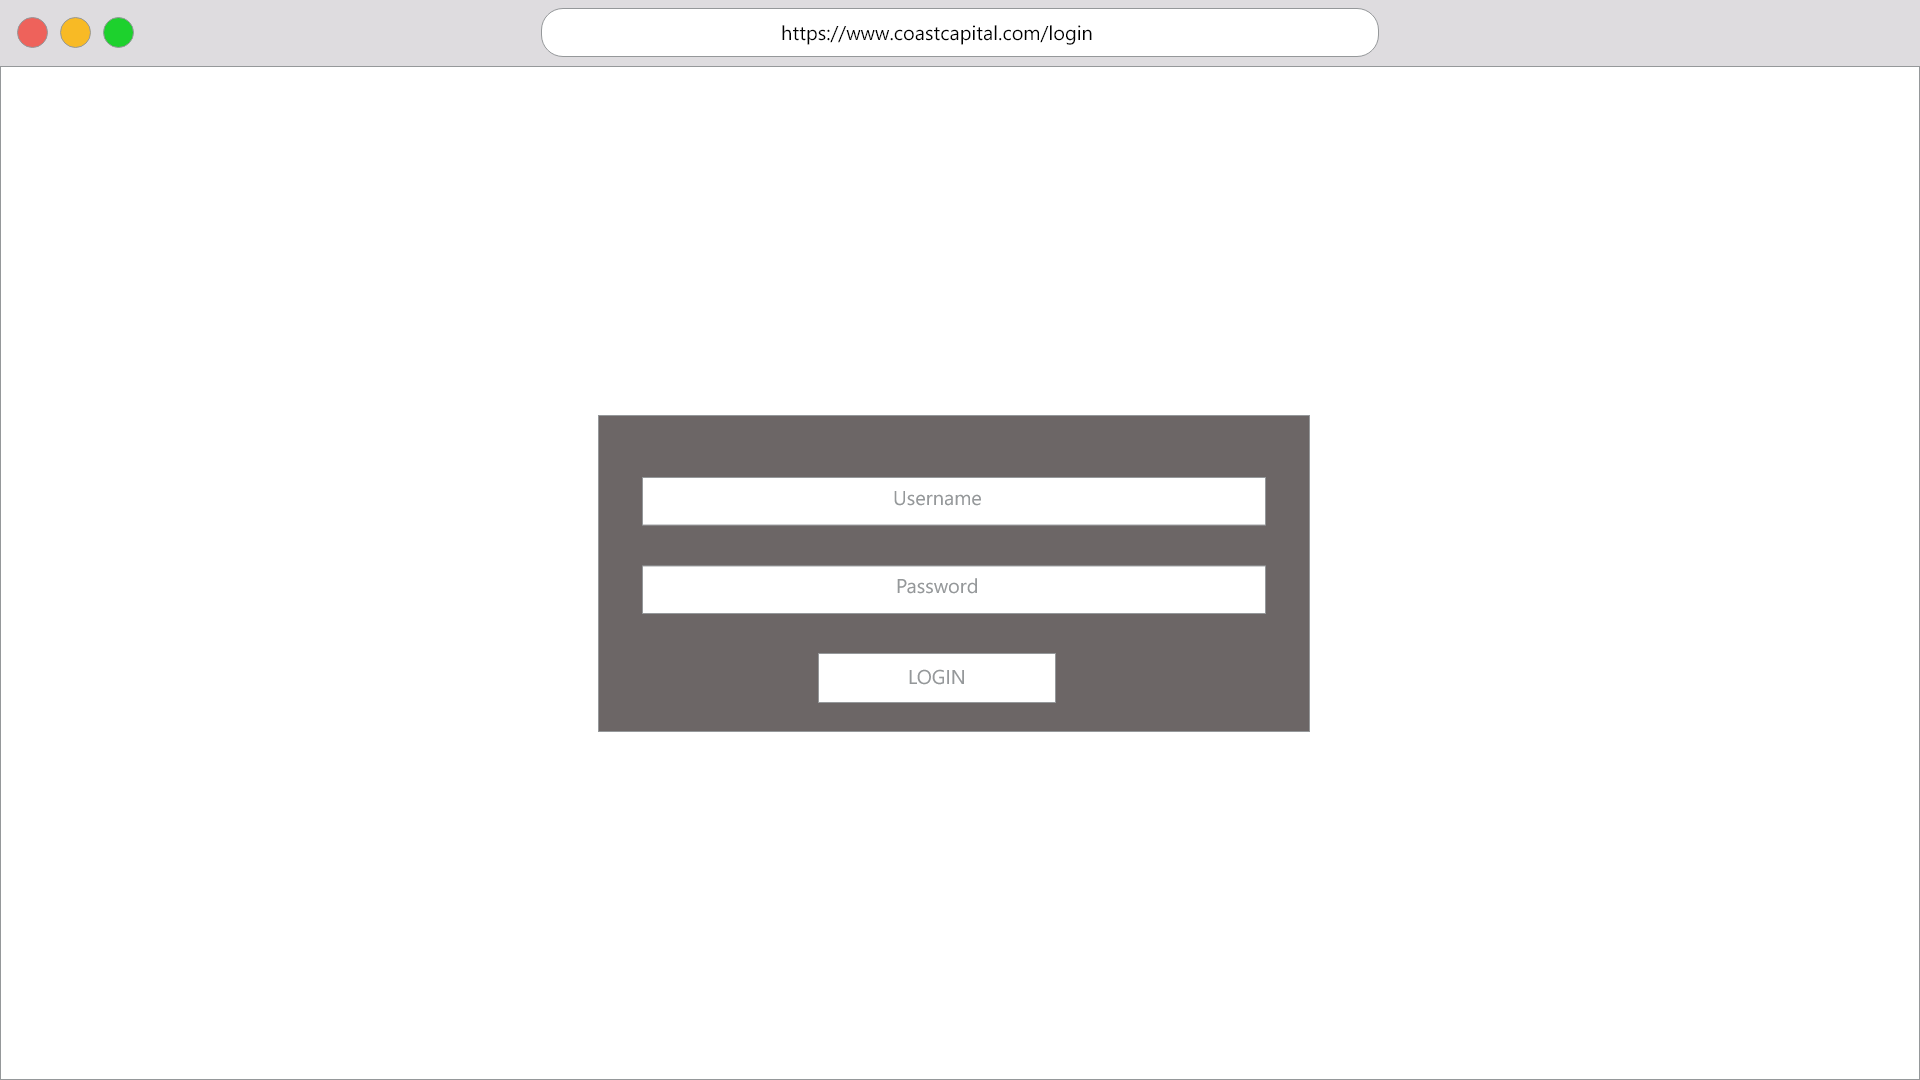
\includegraphics[width=1.0\textwidth]{../design/Login}

The login page is simply designed to allow us to know who is entering the system, and therefore what should be displayed as options once the user logs in.

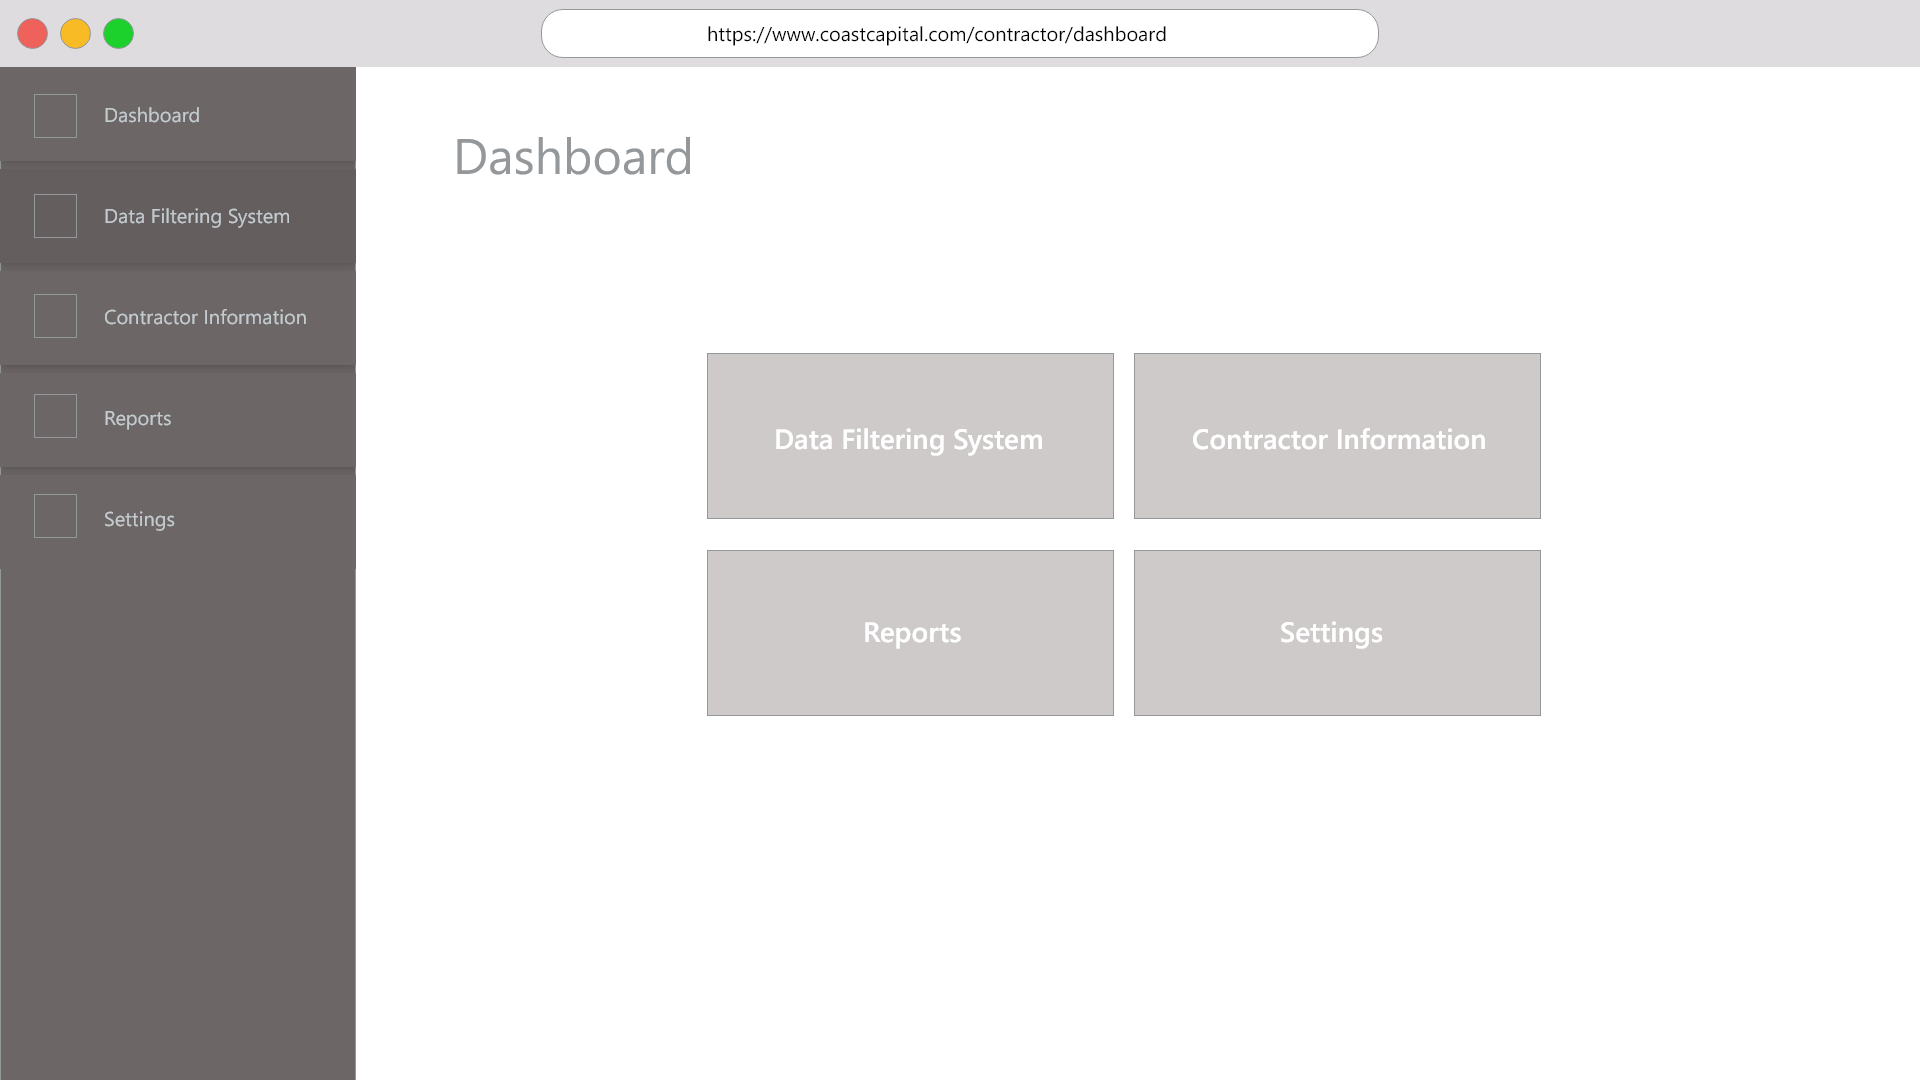
\includegraphics[width=1.0\textwidth]{../design/Dashboard}

The dashboard allows the user to select the type of task they would like to do once logged in. While the same buttons are available on the left navigation panel, this allows the user to cleanly enter the web application, without the landing page overwhelming them with data that would otherwise be the data filtration page. Additional functionality (not shown) could be to have some form of a profile page. 

\includegraphics[width=1.0\textwidth]{"../design/Filter Data"}

The data filtration system works a lot like the excel spreadsheet, by initially providing all the contractor data, until the user filters through, and selects what he or she would like to see. The similarity to the current system they have will provide good learnability, and efficiency in learning the system. 

\includegraphics[width=1.0\textwidth]{"../design/Edit Contractor"}

Users can directly choose to edit a particular tuple, which redirects them to a web-form style page where the fields are auto-populated with the data from the contractor table. Edits can be made to any field (but the field cannot be empty). The option to edit multiple contracts that the contractor is part of is also available. 

\includegraphics[width=1.0\textwidth]{"../design/Add Contractor"}

The user can add contractors to the contractor database. The same web-form that we saw with edit contractors is made available, and there is the option to add multiple contracts for one contractor at one time. This prevents the system from being annoying and frustrating since multiple projects can be added at once. 

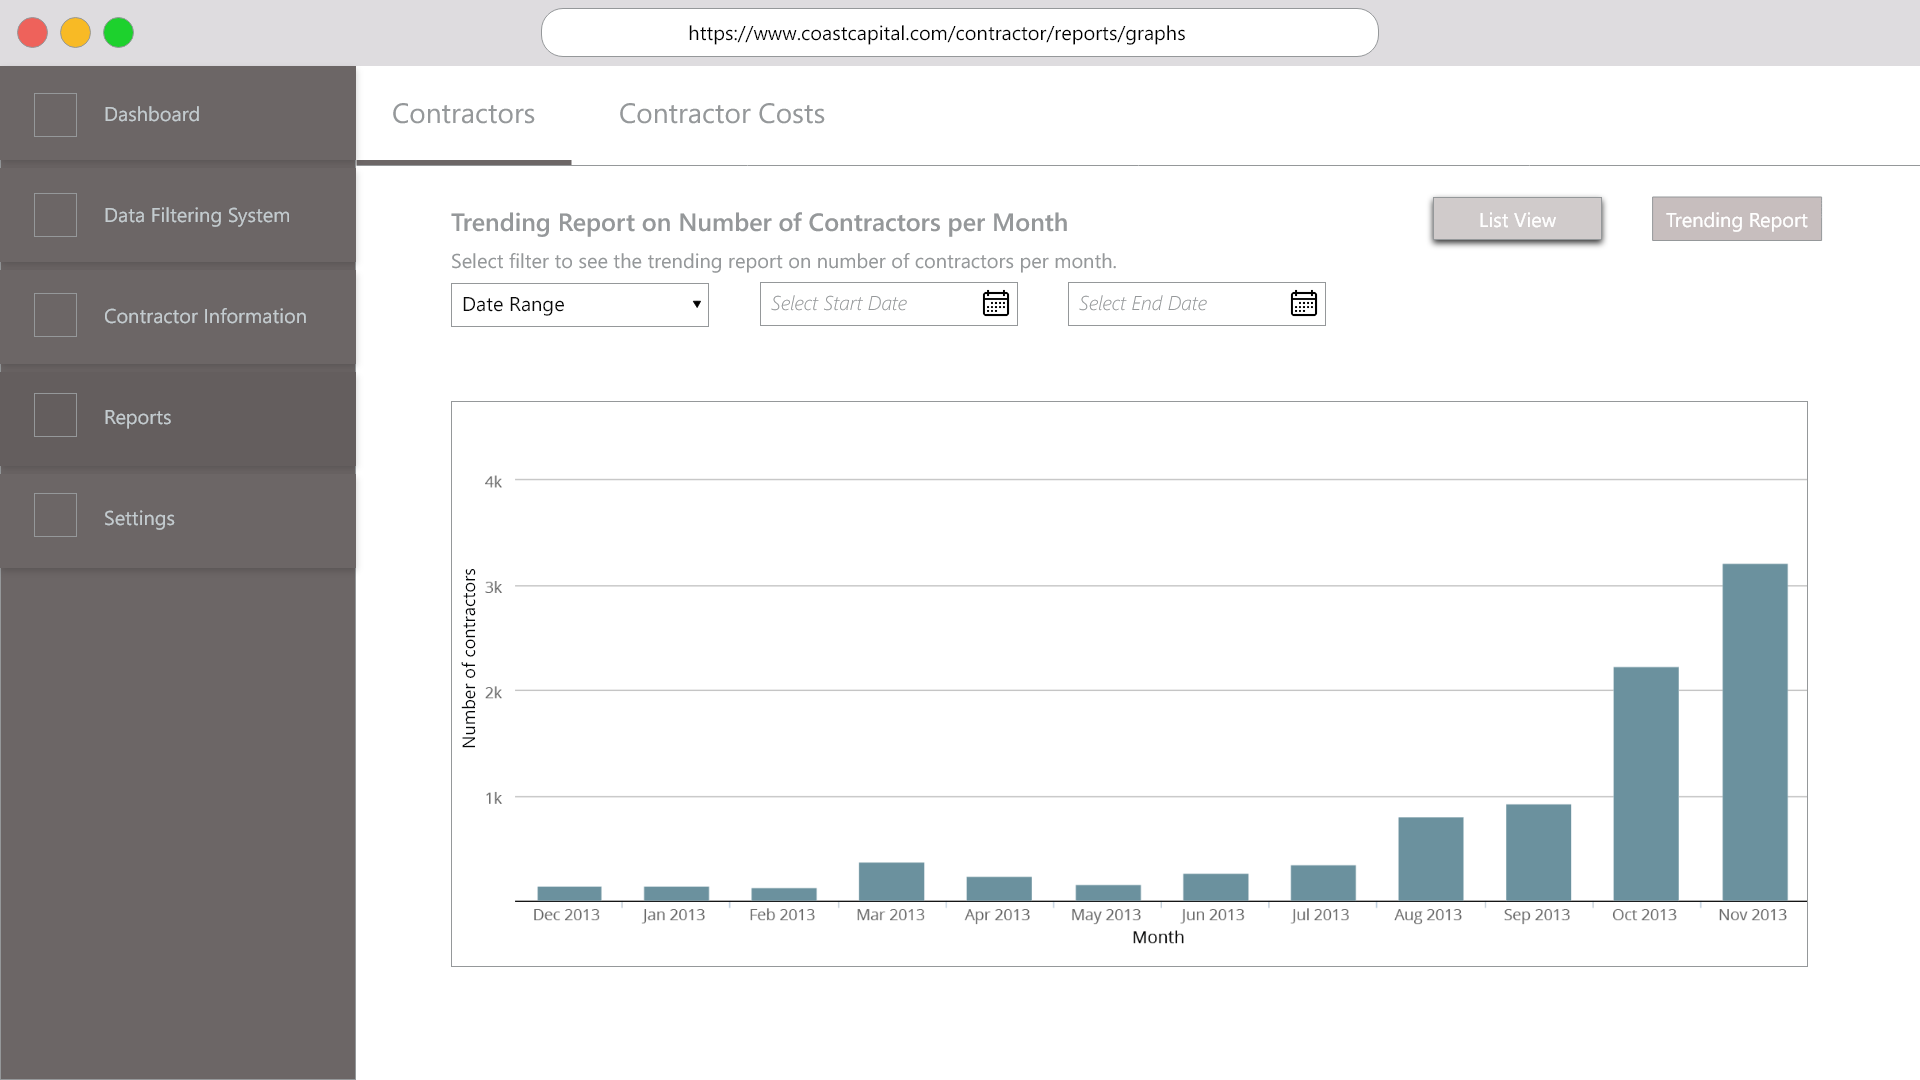
\includegraphics[width=1.0\textwidth]{../design/Report}

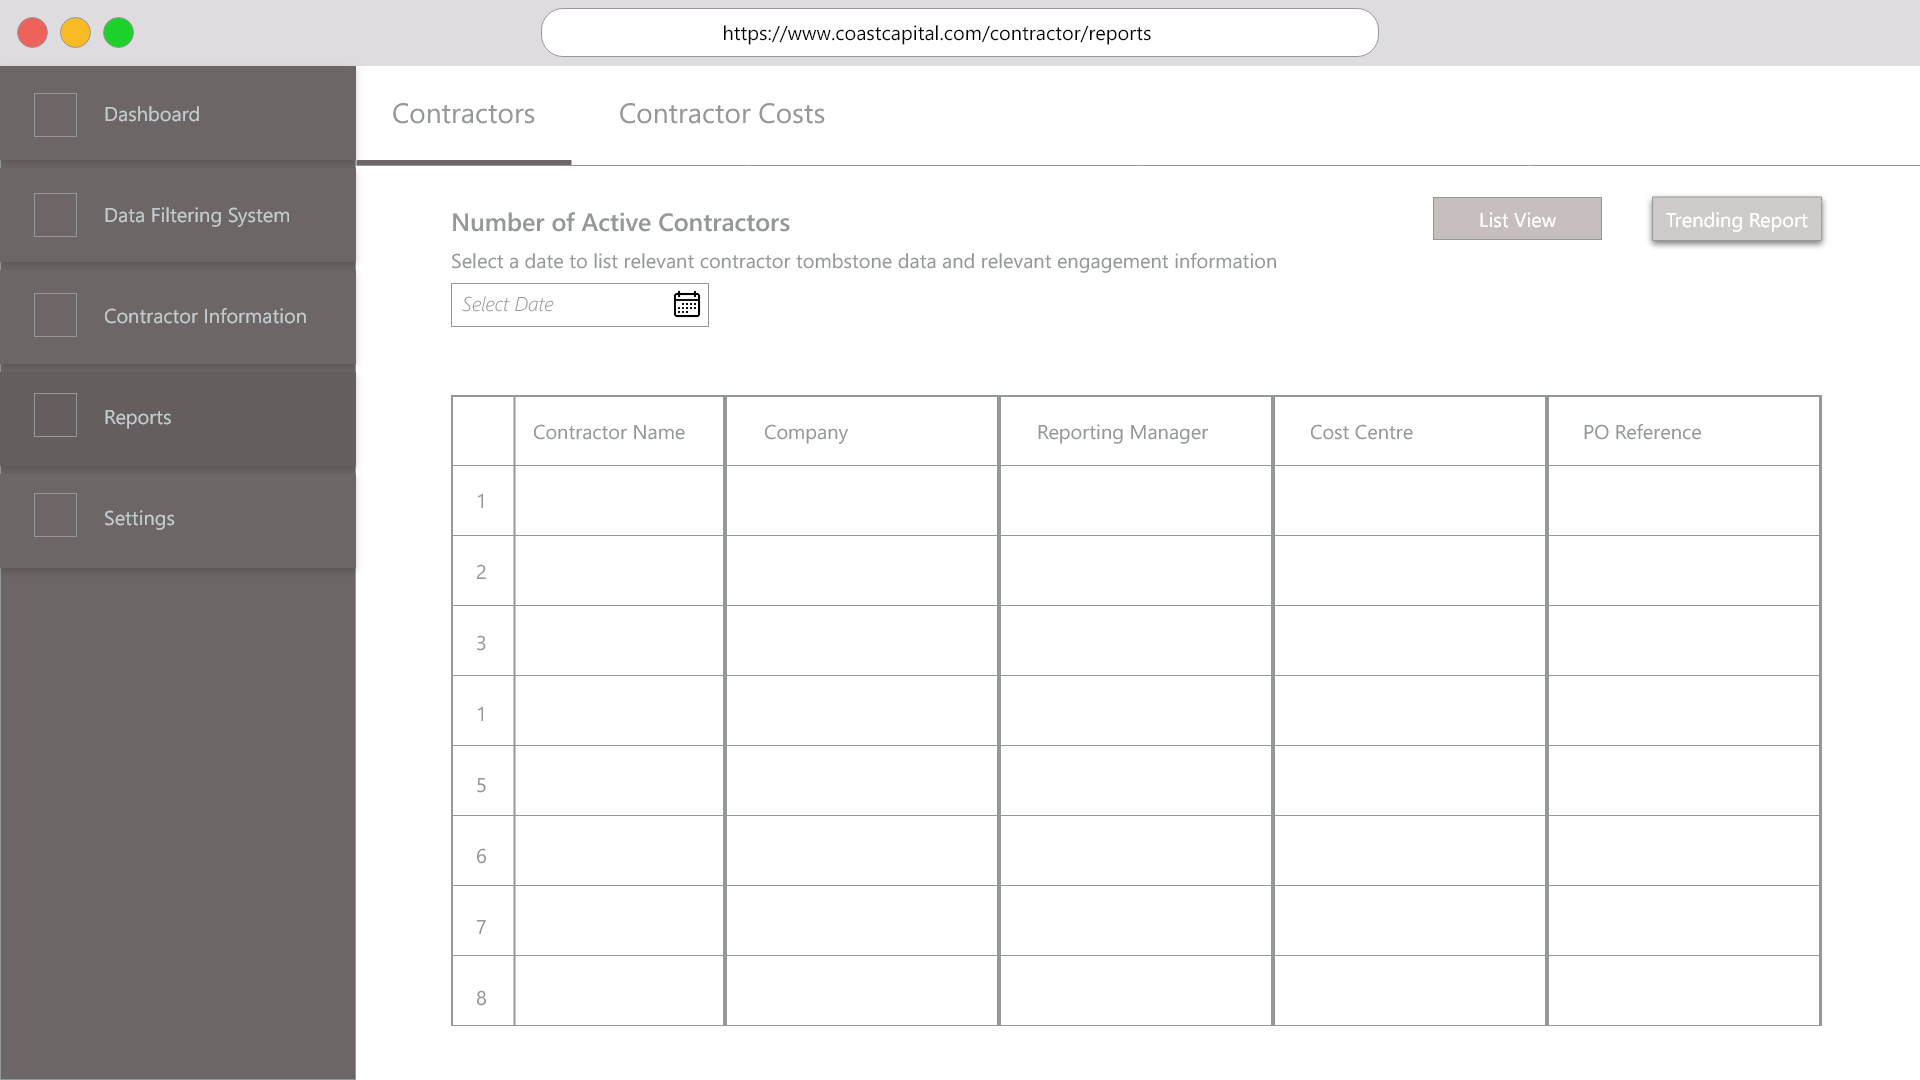
\includegraphics[width=1.0\textwidth]{../design/Report1}

Reports can be generated as lists or as bar graphs. The tab selection on top reduces the clutter, and makes the system very intuitive on what has been selected and what hasn�t. Filtering on the graphs can be done through a drop down menu.

\includegraphics[width=1.0\textwidth]{"../design/Admin Dashboard"}

Admins have an additional dashboard that allows them to maintain various types of data tables. 

\section{Programming Environment}

\subsection{Summary}

We will be using JavaScript, Java and MySQL for this project.

\subsection{Front-End Technology}

\begin{center}
        \begin{table}[!htbp]
        \centering
        \begin{tabularx}{\linewidth}{|| c | L ||}
    \hline
    WebStorm & WebStorm provides great JS developing tools and it�s free for students. \\
    \hline
    JavaScript & The site is interactive, so we will need to use JS. \\
    \hline
    Node.js NPM & We will be using different libraries and packages, and NPM will help with managing them.\\
    \hline
    React & The site will have to be highly interactive and responsive, and React will provide that for us. \\
    \hline
    Redux & To achieve fast response times and avoid further API calls to the tables, Redux will provide a state management tool for us to store the data the first time we receive it. \\
    \hline
    webpack & This tool will be used for module bundling and integrating other tools and libraries (e.g. babel, linters, css loader, etc.) \\
    \hline
    Babel & Since we will be supporting IE11, it is essential for our JS code to be recompiled for compatibility. Babel will be doing that for us. \\
    \hline
    CSS Loader & This library will help us integrate CSS and JS. \\
    \hline
    D3.js & This JS library will help us to visualize graphs and reports. \\
    \hline
    \end{tabularx}
    \end{table}
\end{center}

\clearpage

\subsection{Back-End Technology}

\begin{center}
        \begin{table}[!htbp]
        \centering
        \begin{tabularx}{\linewidth}{|| c || L ||}
    \hline
    IntelliJ & Intellij provides an IDE for developing in a wide variety of languages with excellent support for Java. It also is free for students. \\
    \hline
    DataGrip & DataGrip provides an IDE for developing databases, we will be using this for viewing, creating, and interacting with our SQL database (alongside interaction through Java code). DataGrip is provided free of charge for students.\\
    \hline
    Java & Java is our main programming language for the business logic of our application. \\
    \hline
    MySQL & We will be using MySQL as our relational database management system for storing data, aligning us with Coast Capital�s requirements.\\
    \hline
    Amazon RDS & Amazon RDS (Relational Database Service) is where we will be hosting our MySQL database. \\
    \hline
    AWS Elastic Beanstalk & AWS (Amazon Web Services) Elastic Beanstalk is where we will be hosting our web application. \\
    \hline
    Spring & We will be using the Java Spring framework for creating REST endpoints as well as for its dependency injection features. \\
    \hline
    \end{tabularx}
    \end{table}
\end{center}

\clearpage

\section{Prdouction and Test Environments}

\subsection{Front-End Technology}

\begin{center}
        \begin{table}[!htbp]
        \centering
        \begin{tabularx}{\linewidth}{|| c | L ||}
    \hline
    Selenium & Selenium is a tool that allows us to automate testing, eliminating the risk of forgetting to test through manual testing, and speeding up the process of an otherwise menial task. It also allows for frequent regression testing.  \\
    \hline
    Mocha & Mocha is very useful for testing asynchronous calls in JavaScript. It uses node.js and is useful for mapping uncaught exceptions to the correct test cases. \\
    \hline
    Chai & Chai is a great extension for Mocha which will give us more in-depth unit testing abilities.\\
    \hline
    Sinon & In order to test API calls from the front-end, Sinon will give us a fake server, function spies, fake responses, etc.\\
    \hline
    \end{tabularx}
    \end{table}
\end{center}

\clearpage

\subsection{Back-End Technology}

\begin{center}
        \begin{table}[!htbp]
        \centering
        \begin{tabularx}{\linewidth}{|| c | L ||}
    \hline
    JUnit & We will be using JUnit for unit testing all of our Java code. \\
    \hline
    Mockito & We will be using Mockito to mock certain aspects of our application to allow for easier unit testing (such as mocking database connections). \\
    \hline
    \end{tabularx}
    \end{table}
\end{center}

\section{Software Architecture}

We visualized the back-end and front-end architecture using a UML Class Object and System Flow diagram. The UML diagram helps us to visualize the structure of the various classes and their attributes. We have all the different kinds of tables implementing the table interface since each of them has similar functionality even though they have different attributes. The admin class extends the user class and has extra functionalities for the admin specific tasks.

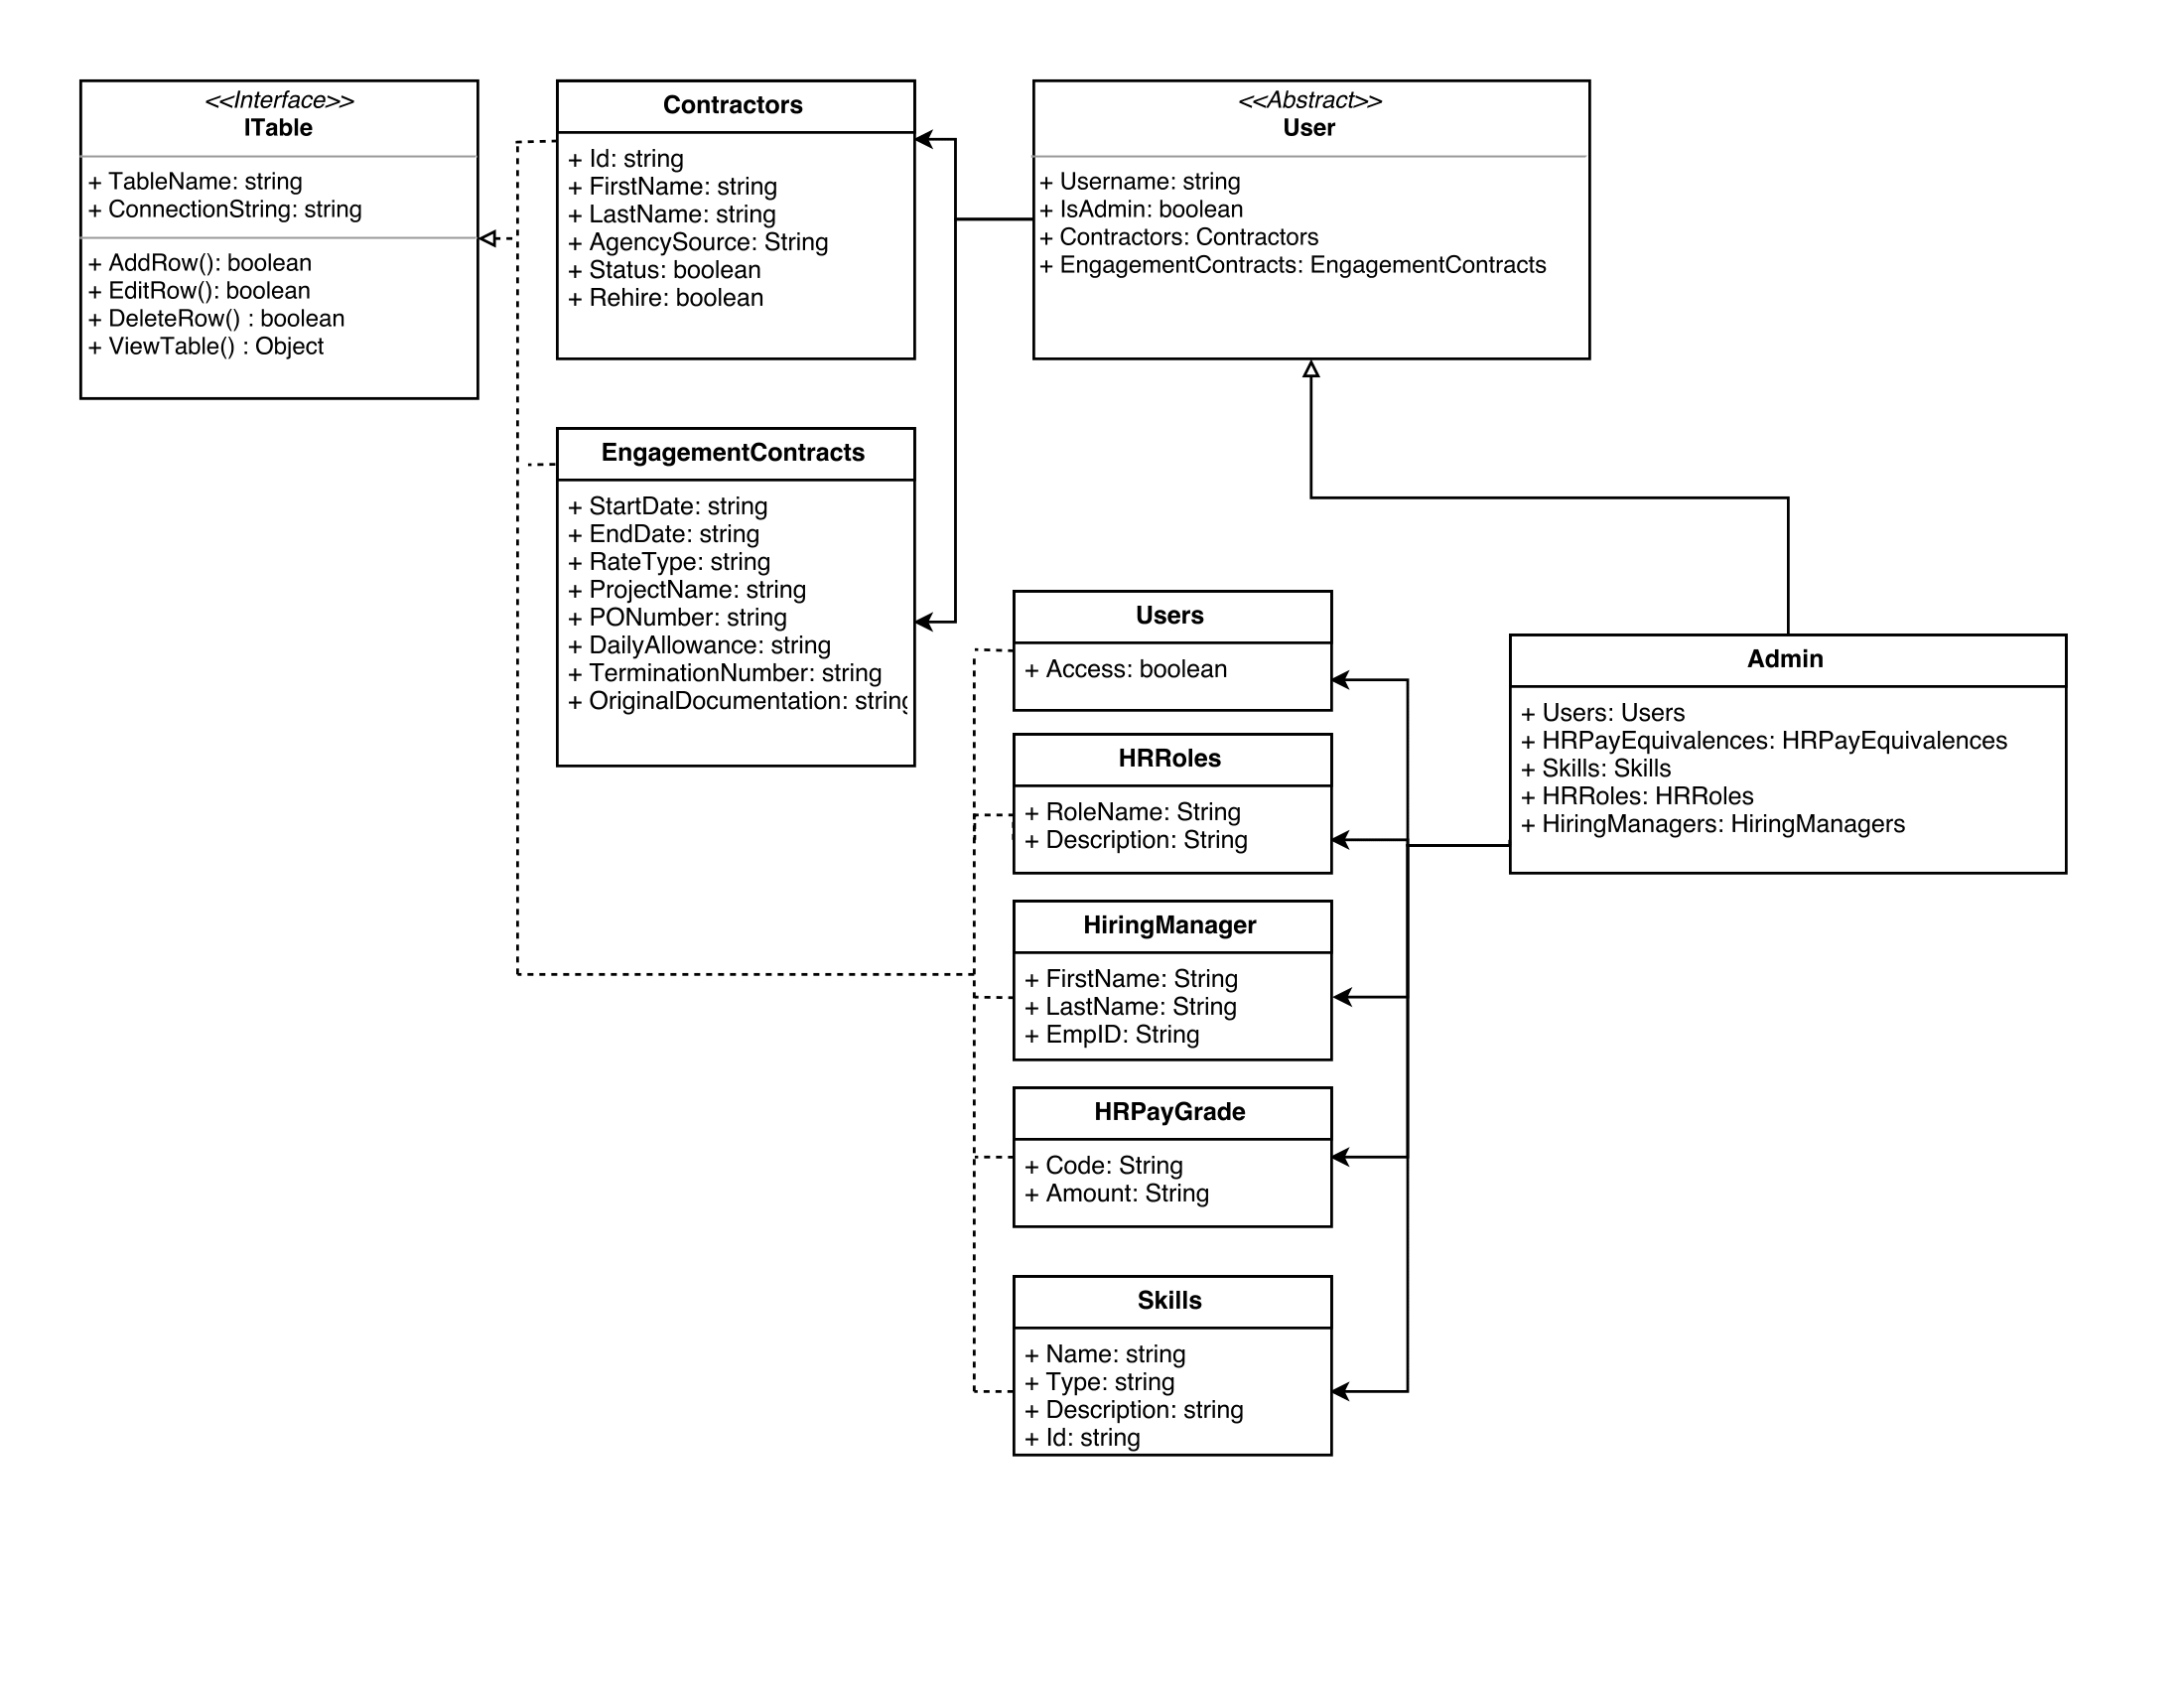
\includegraphics[width=1.0\textwidth]{../design/uml-1}

The system flow shows the communication between the frontend and backend as well as the structure of the frontend code. As shown in the diagram below, each user is validated while logging in which determines if they get administrative access. The administrator has the right to add, edit, or delete users. All users in the system can add and edit contractors, view and filter tables or generate reports/graphs. The admin's management of other tables isn't shown explicitly in the diagram but pls refer to the mock up screen

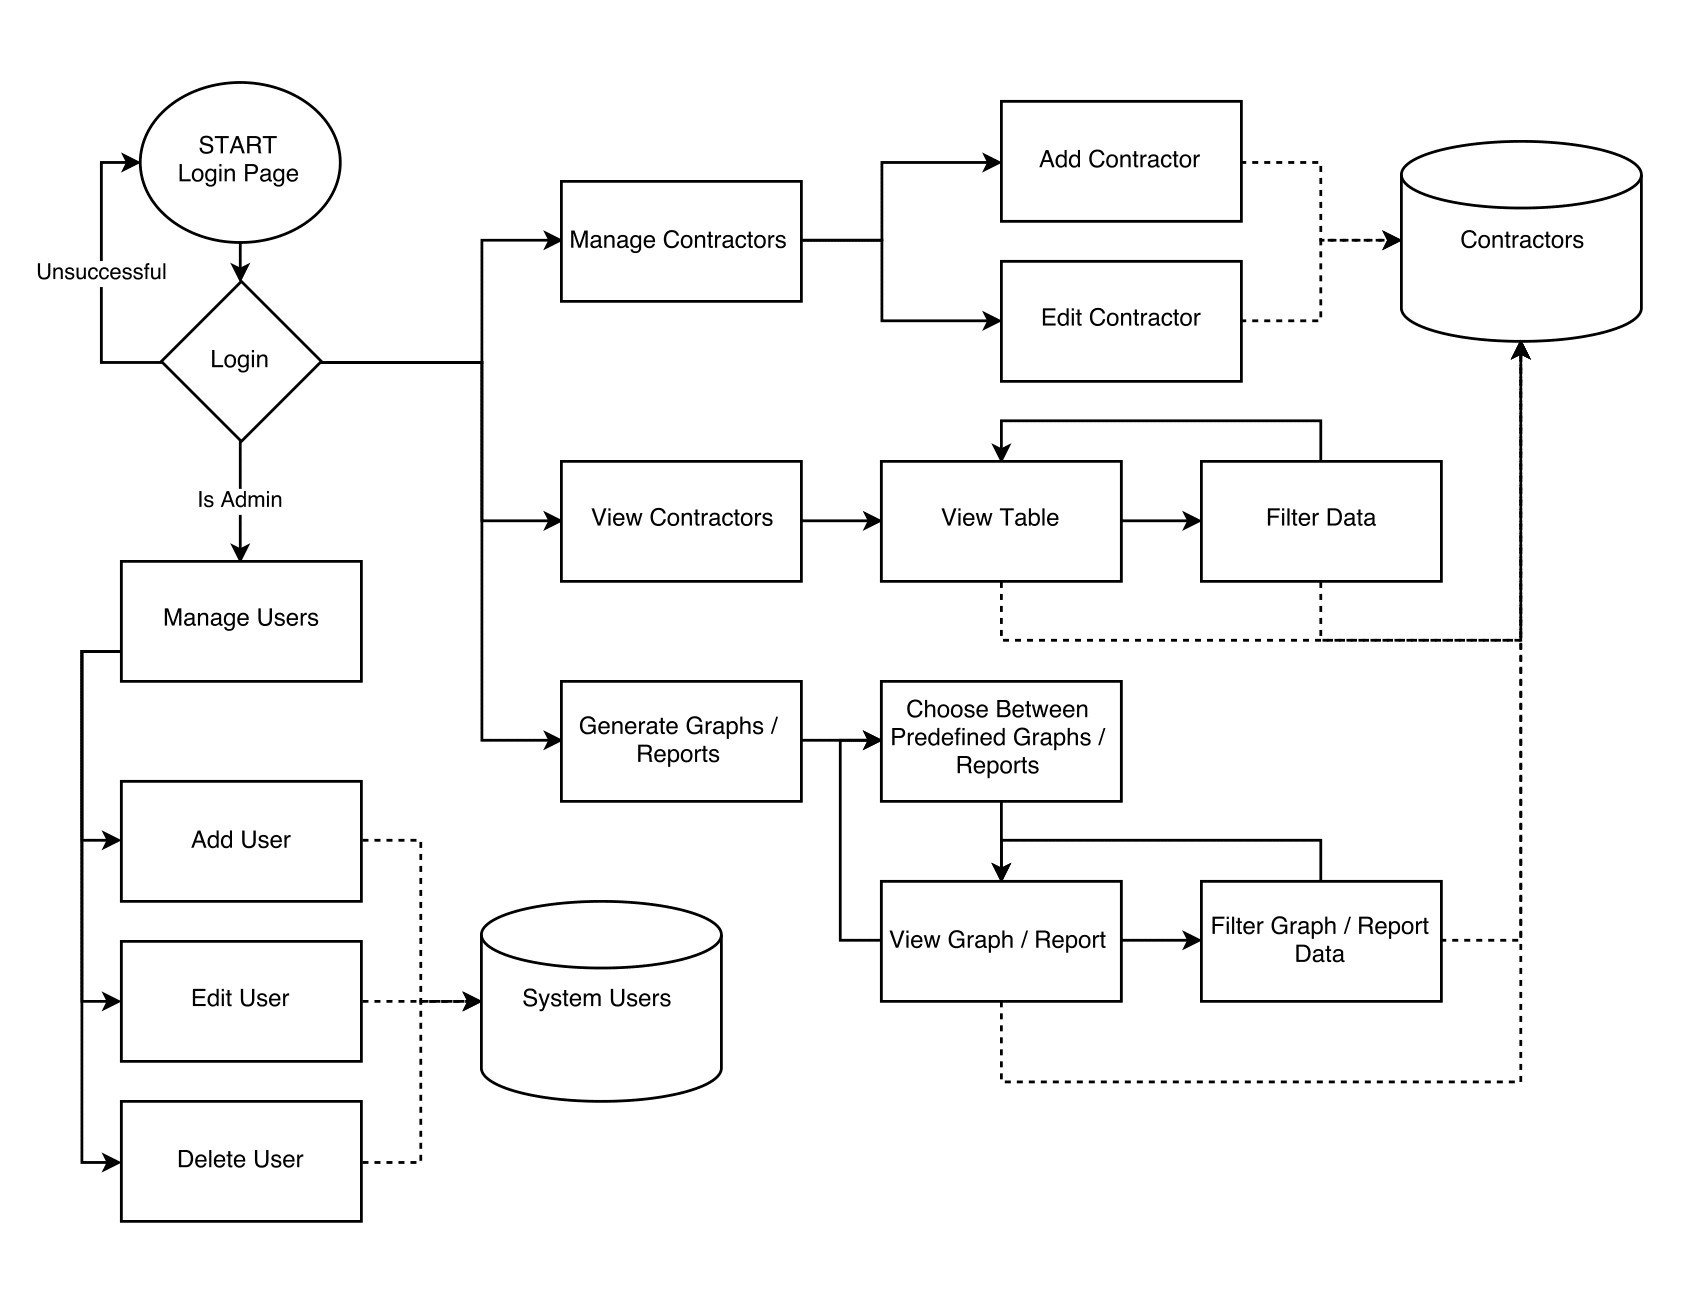
\includegraphics[width=1.0\textwidth]{../design/FlowChart}

\section{Data Design}

\subsection{ER Diagram}

Our ER diagram showcases the data and relationships we will be capturing within our database. The ER diagram shows the cardinality of relationships between tuples and also highlights the primary keys as well as other attributes each tuple will contain. It is from this ER diagram that a normalized database schema was created.

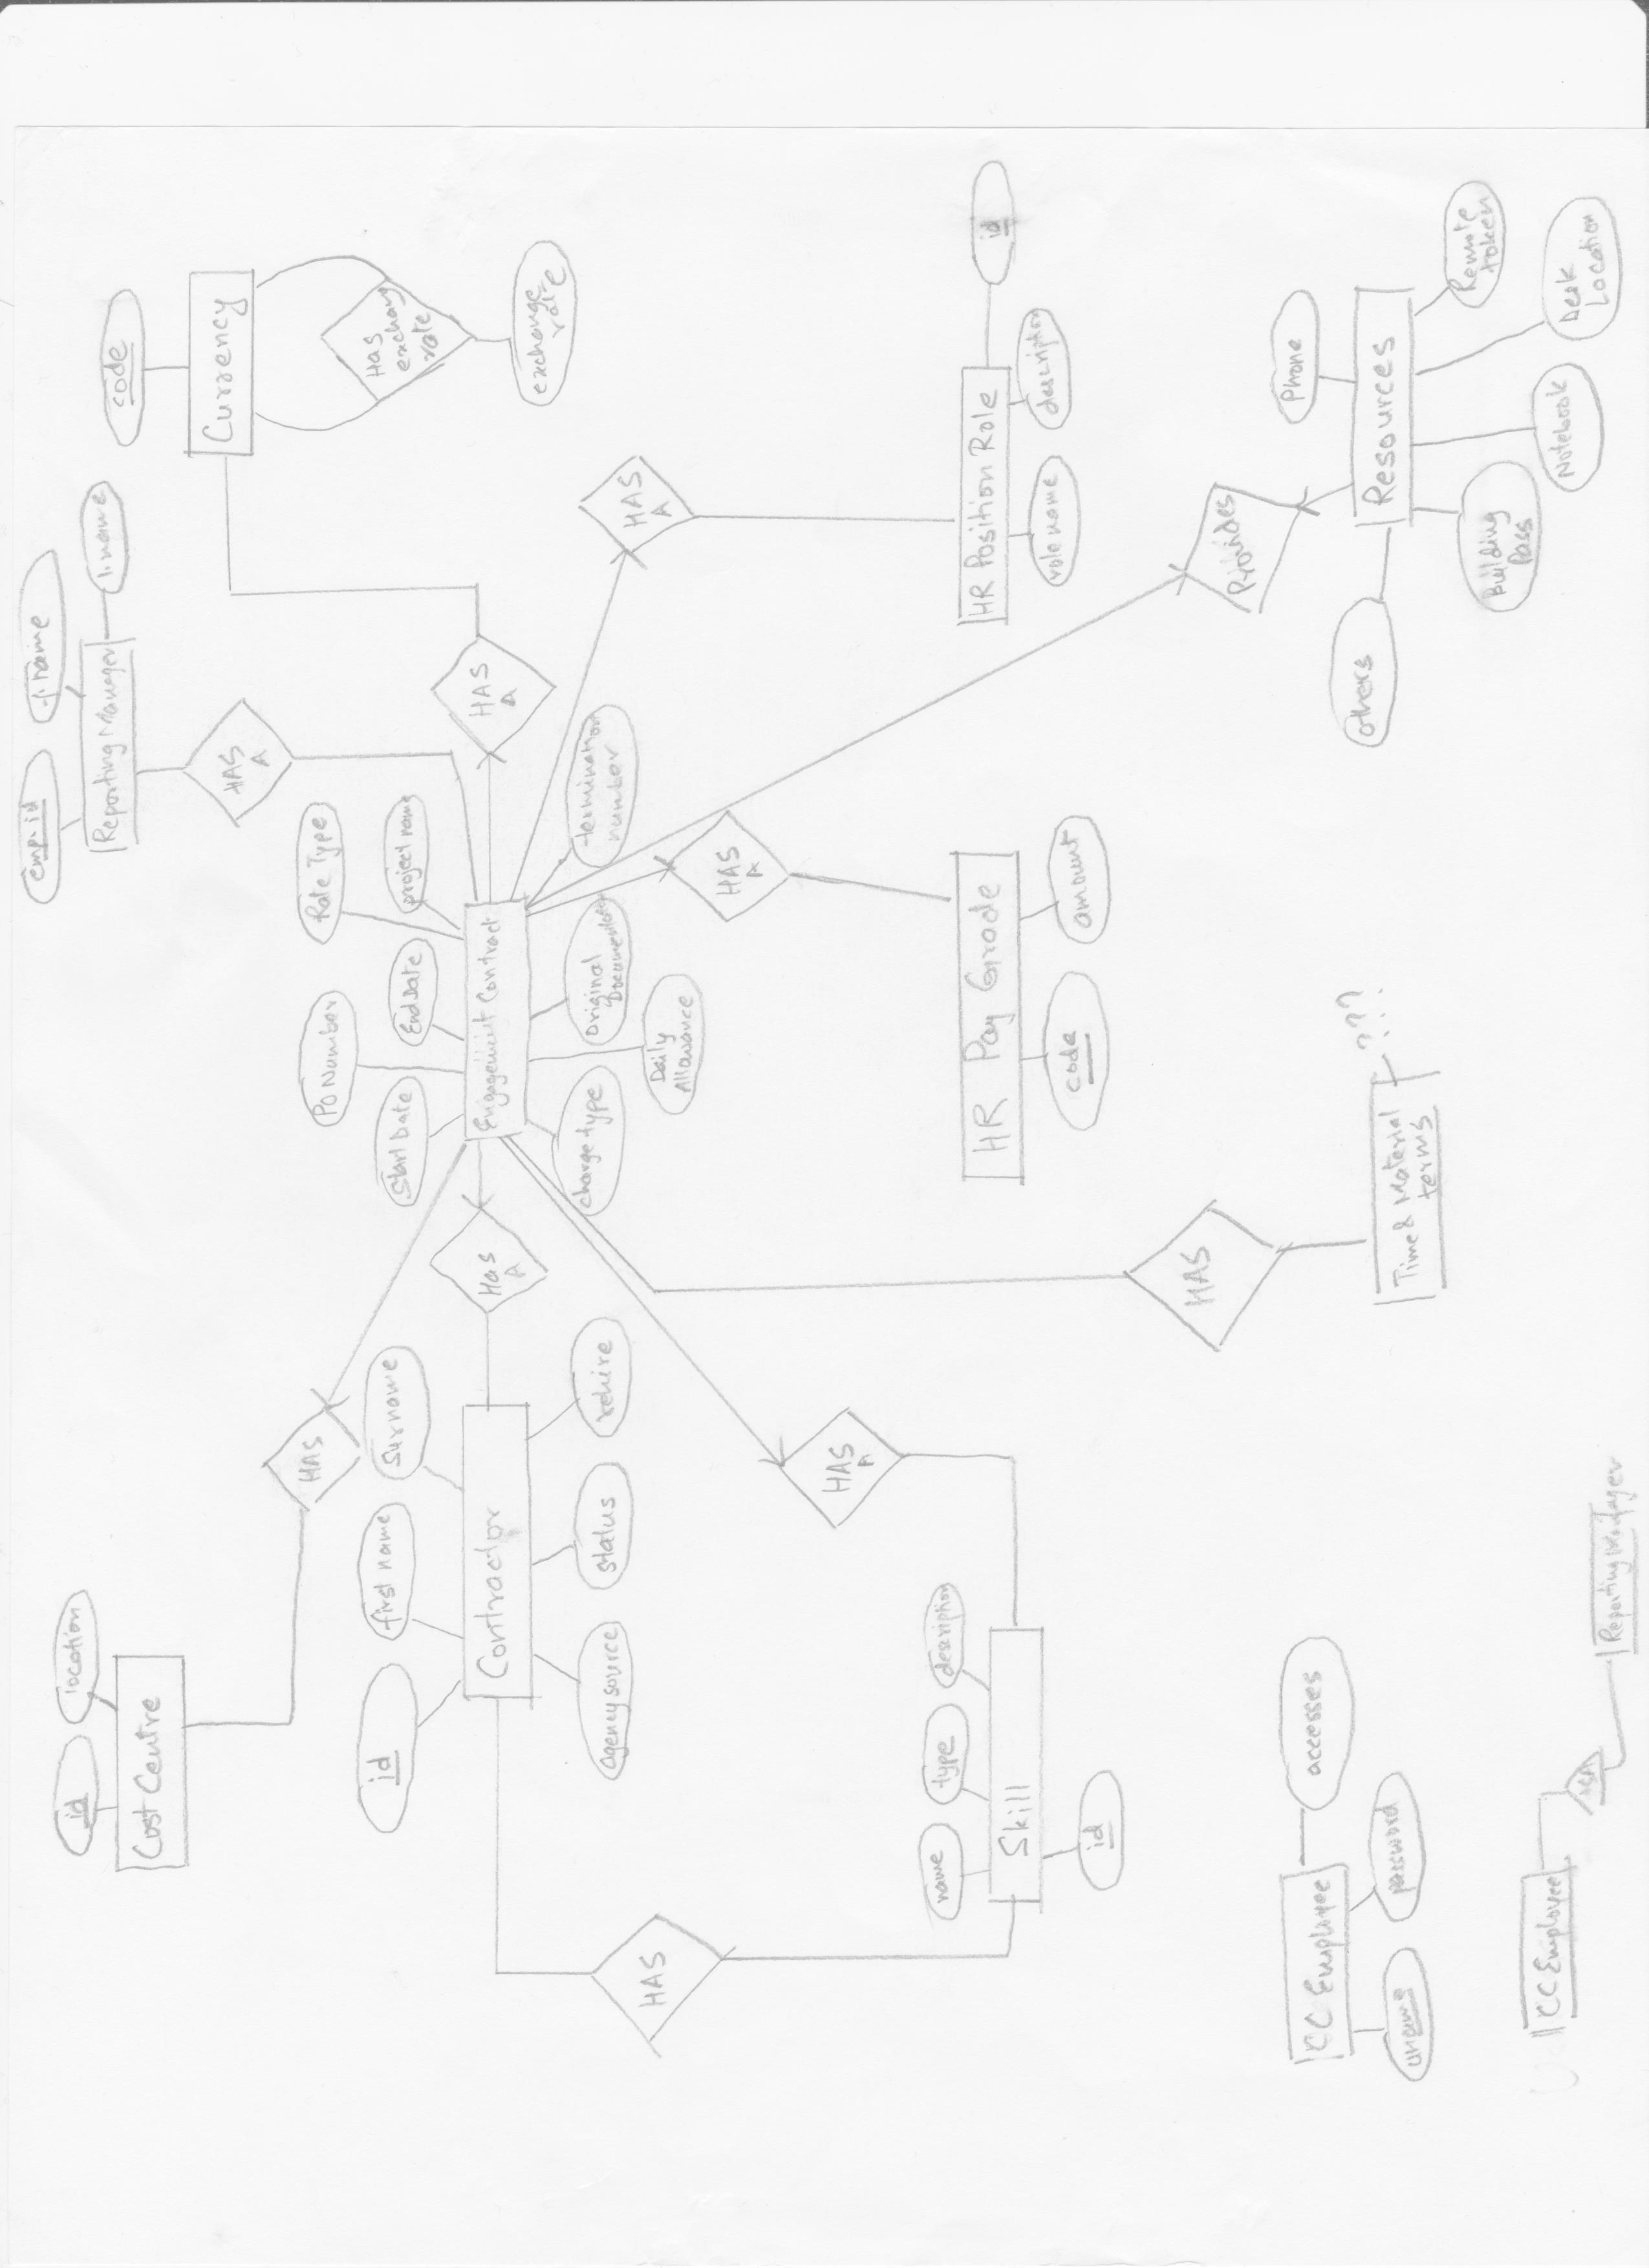
\includegraphics[width=0.7\textwidth, angle =270]{../design/er}

\subsection{Normalized Database Schema}

Here is the list of tables:

(Undelrined attribute is the primary key whereas bolded attribute is a foreign key)

\begin{enumerate}
    \item User (\underline{username}, password, permissions)
    \item Contractor(\underline{id}, firstName, surname, agencySource, status, rehire)
    \item EngagementContract(\underline{id}, startDate, endDate, rateType, projectName, chargeType, dailyAllowance, originalDocumentation, terminationNum, \textbf{contractorId, resourceId, hrPositionId, hrPayGradeId,  costCenterId, reportingManagerUserId, currencyCode, mainSkillId})
    \item SkillProvided(\underline{id}, \textbf{contractorID}, name, type, description)
    \item ResourceProvided(\underline{id}, \textbf{engagementID}, phone, remoteToken, buildingPass, notebook, deskLoc, others)
    \item HRPositionRole(\underline{id}, roleName, description)
    \item HRPayGrade(\underline{code}, startAmount, endAmount)
    \item CostCenter(\underline{id}, location)
    \item Currency(\underline{code}, location)
    \item FXRate(\textbf{\underline{curCode1}, \underline{curCode2}}, rate)
\end{enumerate}

The normalized database schema shows the tables required for capturing all of the information used by our application. The schema has primary keys underlined and foreign keys bolded. The database is normalized into third normal form to allow for fast access of necessary data and to reduce redundant data stored within the database. 

\section{API Design}

\subsection{API Calls-Internal}

\begin{enumerate}
        \item login(username, password) - Allows a user to login to the web application.
        \item createNewUser(User) - Allows an admin user to create a new user in the database.
        \item updateUser(User) - Allows an admin user to update an existing user in the database.
        \item deleteUser(User) - Allows an admin user to delete an existing user from the database.
        \item fetchContractorData(Contractors) - Fetches relevant contractor data for the given contractor.
        \item fetchAllActiveContractorData() - Fetches data relating to all active contractors and their engagement contracts.
        \item fetchAllContractorData() - Fetches data relating to all contractors (active and inactive) and their respective engagement contracts. 
        \item updateContractor(Contractor) - Updates data relating to the given contractor in the database. 
        \item addContractor(Contractor) - Adds the given contractor to the database. 
        \item updateEngagementContract(EngagementContracts) - Updates data relating to the given engagement contract.
        \item addEngagementContracts(List\textless EngagementContracts\textgreater ) - Adds the given EngagementContract(s) to the database.
        \item updateSkills(Skills) - Updates data relating to the given skill in the database.
        \item addSkills(Skills) - Adds the given skill to the database.
        \item deleteSkills(Skills) - Delets the given skill in the database.
        \item updateHRPayGrade(HRPayGrade) - Updates the given HRPayGrade in the database
        \item addHRPayGrade(HRPayGrade) - Adds the given HRPayGrade to the database.
        \item deleteHRPayGrade(HRPayGrade) - Deletes the given HRPayGrade from the database.
        \item updateHRRole(HRRoles) - Updates the given HRRole in the database.
        \item addHRRole(HRRoles) - Adds the given HRRole to the database.
        \item deleteHRRole(HRRoles) - Deletes the given HRRole from the database.
        \item updateHiringManager(HiringManager) - Updates the given HiringManager in the database.
        \item deleteHiringManager(HiringManager) - Deletes the given HiringManager in the database.
        \item addHiringManager(List\textless HiringManager\textgreater ) - Adds the given HiringManager(s) to the database.
\end{enumerate}

\subsection{API Calls-External}

We will be calling the fixer.io API to get the latest currency exchange rates so that a user does not have to update the currency exchange rates manually. Specifically, we will be using a GET call to http://api.fixer.io/latest?base=CAD\&symbols=USD to get the exchange rate between the Canadian dollar and the United States dollar. This API will be automatically called once per day to update the FXRate table to the latest exchange rate. 

\section{Algorithms}

We will not be using any complex algorithms in our code. One of the more complicated processes will involve implementing a state management environment (Redux) for front-end. The state will be created once a session starts, and it will feed each React component the data it needs to render. When the user interacts with the page, actions will be dispatched to update the state of the app accordingly. These interactions can be as small as typing something into a form or as big as requesting data from the back-end.

\section{Notable Tradeoffs}

\begin{enumerate}
    \item Since we are using AWS for our hosting needs opposed to setting up our own physical server infrastructure, we have less control over the actual hardware used to host our server. However, setting up our server on AWS is a lot faster and easier than setting up our own infrastructure and AWS already has scaling built in so we do not have to worry about those issues. Furthermore, we do not have to deal with physical server maintenance as Amazon takes care of that for us.
    \item When filtering tables/graphs, the client will take care of it instead of calling an API to ask the back-end to do it. It will be faster and easier to manage because there will be fewer API calls. However, the front-end code will be more complicated and if the data is very big, filtering can be slow.
    \item When filtering tables/graphs, the client will take care of it instead of calling an API to ask the back-end to do it. It will be faster and easier to manage because there will be fewer API calls. However, the front-end code will be more complicated and if the data is very big, filtering can be slow.
    \item For visualization, we decided to use d3.js as compared to other APIs since it helps us to keep the data secure rather than sharing it with an external server. However, this also means more complicated code in the front-end.
\end{enumerate}

\section{Notable Risks}

\begin{enumerate}
    \item One notable risk is using AWS to host our database and web application, if AWS were to go down then our web application will not function. However, AWS provides a guarantee of 99.95\% Monthly Uptime Percentage so the likelihood that AWS will go down is very low. 
    \item Another risk is if we do not implement safety prompts or an automatic session expiry for the user. Implementing safety prompts in the UI would ensure that the user does not accidentally change data and an automatic session expiry would ensure that the user does not expose sensitive data.
\end{enumerate}

\end{document}
